\subsection{One-sided hypothesis tests (special topic)}

\Comment{This section needs a lot of work. Maybe it shouldn't
    even be mentioned? It absolutely should not be so aggressive
    and also much shorter.}

\emph{One-sided hypothesis testing is an advanced
    topic due to the nuances around using this method.
    You need only read this section if you are ever asked
    to complete a \term{one-sided hypothesis test}.} \\

So far we've only considered what are called \term{two-sided
hypothesis tests}, where we care about detecting whether $p$
is either above or below some null value $p_0$.
There is a second type of hypothesis test called a
\term{one-sided hypothesis test}.
For a one-sided hypothesis test,
the hypotheses take the form of one of the following:
\begin{enumerate}
\item If we truly only care about detecting if the population
    parameter were \emph{less than} some value~$p_0$:
  \begin{description}
  \item[$\mathbf{H_0}$:] $p = p_0$.
  \item[$\mathbf{H_A}$:] $p < p_0$. The parameter $p$ is less
      than the null value $p_0$.
  \end{description}
\item If we truly only care about detecting if the population
    parameter were \emph{more than} some value~$p_0$:
  \begin{description}
  \item[$\mathbf{H_0}$:] $p = p_0$.
  \item[$\mathbf{H_A}$:] $p > p_0$. The parameter $p$ is more
      than the null value $p_0$.
  \end{description}
\end{enumerate}
Notice that we still write the null hypothesis using an
equality in the one-sided hypothesis test case.

While this one-sided test approach is common in many
introductory statistics textbooks, these tests create
some philosophical problems that we lightly touch on
here. In some instances, such as in clinical trials
where we might test out whether a new drug is effective,
one-sided tests are banned.

\begin{example}{Suppose we're on a business team that is
    considering whether to go into a new market. If they
    more than 20\% of the buyers would be interested in
    their product, they will move into that market. If not,
    they will not enter the market. Set up an appropriate
    one-sided hypothesis test for this situation.}
  We care about determining whether there is convincing
  evidence that the population proportion $p$ is greater
  than 20\%, so we make this our alternative hypothesis
  and use equality for the null:
  \begin{description}
  \item[$\mathbf{H_0}$:] $p = 0.20$
  \item[$\mathbf{H_A}$:] $p > 0.20$
  \end{description}
\end{example}

\begin{example}{The business runs a survey of a simple
    random sample of 400 people in the market of interest,
    and 21\% of the people express interest in the
    business' product. Will (should) the business decide
    to enter the market?}
    \label{business_one_sided_20_21}
  There is only one difference in evaluating a one-sided
  hypothesis test vs a two-sided hypothesis test: how to
  compute the p-value.
  In a one-sided hypothesis test, we compute the p-value as
  the tail area in the \emph{direction of the alternative
  hypothesis}. In this example, here we only care about
  detecting whether $p$ is greater than 20\%, so we compute
  the upper tail area and use this as the p-value.
  \begin{description}
  \item[Conditions.] The data come from a simple random sample
      and the success failure condition is satisfied
      ($n \times p_0 = 80$ and $n \times (1 - p_0) = 320$).
  \item[Compute.] Compute the standard error using the null
      value: $SE_{\hat{p}} = \sqrt{0.2 (1 - 0.8) / 400} = 0.01$.
      Next compute
      $Z = \frac{\hat{p} - p_0}{SE_{\hat{p}}}
         = \frac{0.21 - 0.20}{0.01}
         = 1.00$.
      Finally, compute the tail area where $p > 0.20$,
      we consider the upper tail:
      \begin{center}
      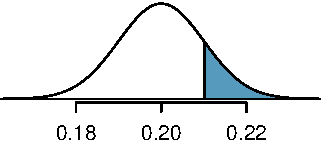
\includegraphics[width=0.3\textwidth]{ch_inference_for_props/figures/business_one_sided_20_21-p_value/business_one_sided_20_21-p_value}
      \end{center}
      We can find the p-value from software or using the
      normal probability table: 0.1587.
  \item[Conclude.] Since the p-value is greater than 0.05,
      we do not find convincing evidence that the fraction
      of the market that's interested in the company's
      product is greater than 20\%. In this case, the
      company would not enter the market.
  \end{description}
\end{example}

There's a piece of human behavior that we left off in
Example~\ref{business_one_sided_20_21}: the company
would not have entered the market \emph{yet}. One-sided
hypothesis tests work well in isolation. However,
they also define not just a decision but what we can
\emph{learn} from the data, if we are to be thoughtful
about our analysis. %controlling Type 1 Errors.
In the next example, we consider the hypothetical
situation where the survey data came back with
a much smaller percent.

%The one-sided hypothesis test presented in
%Example~\ref{business_one_sided_20_21}
%didn't throw up any surprises when it comes to
%questioning whether a one-sided test was reasonable
%
%In Example~\ref{business_one_sided_20_21},
%we considered some data and evaluated the
%one-sided test. However, the examples that follow will dive
%into the logic and philosophy behind one-sided tests and
%whether we can be robotic enough to apply them properly.

\begin{example}{Suppose the survey had actually come back
    with a result that only 7\% of the 400 people were
    interested in their product. In this case, the Z-score
    would have been $Z = -13$. This corresponds to a lower
    tail area of very nearly~0 and an upper tail are of
    very nearly~1.
    How would we correctly interpret this finding when using
    the one-sided alternative hypothesis that $p > 0.20$?}
    \label{business_one_sided_20_7}
  In this one-sided analysis, the p-value would be larger
  than 0.05, and we would simply conclude that we do not
  have strong evidence that the true proportion is greater
  than 20\%.
  
  This is the only conclusion we can make. Our p-value
  doesn't say \emph{anything} about that the result went
  in completely the opposite direction.
\end{example}

\begin{example}{Suppose the company board saw the
    hypothetical survey results from
    Example~\ref{business_one_sided_20_7}
    where the survey findings were that only 7\% of
    the 400 surveyed people were interested in the product.
    How do you think they would interpret those results?}
    \label{business_one_sided_20_7-exec_interpretation}
  The board is probably going to feel comfortable with
  their decision to not enter the market, as they should
  since the p-value is large. However, they may now believe
  the actual proportion to be notably \emph{less than}
  20\%. Unfortunately this is not a valid statistical
  conclusion if we are using a one-sided test: we should
  not attempt to describe or infer the magnitude of the
  difference in the opposite direction of a one-sided
  $H_A$ since this means we are actually running a
  two-sided test.
\end{example}

\emph{You can't have your cake and eat it, too.}
Using a one-sided test to get a slightly smaller p-value
\emph{if} the data goes in the direction of interest means
we cannot later change our minds and make an assertive
conclusion in the opposite direction.
Our natural human tendencies to learn from data and use that
knowledge in the future will generally undermine the validity
of a one-sided hypothesis test. That is, unless there is
an astoundingly good reason and special situation,
only use two-sided tests.
We will not present any additional one-sided scenarios
in this textbook due to the problems we've outlined here,
and because we haven't been able to outline a situation
where this arose.
%even in our
%contrived example where we attempted to set up a situation
%where a one-sided test would be appropriate, we've
%stumbled into a reason why it would actually \emph{not}
%be appropriate.

\begin{termBox}{\tBoxTitle{The risk of flipping
    a one-sided test to a two-sided test inflates
    the Type 1 Error}
  We've been working very hard to build a rigorous
  system for analyzing data. If we introduce the risk
  of flip-flopping into that system, we undermine the
  the principles we're using in statistics.}
\end{termBox}

\begin{example}{
    In Section~\ref{basicExampleOfStentsAndStrokes},
    we encountered an example where doctors were interested
    in determining whether stents would help people were at
    a high risk of stroke.
    The researchers believed the stents would help.
    Unfortunately, they did not, and the study found strong
    evidence that patients who received stents actually did
    worse.
    Why was using a two-sided test so important in
    this context?}
  Before the study, researchers strongly believed that stents
  would, at worst, help patients. Had they used a one-sided
  test, they couldn't have legitimately identified the strong
  evidence that the stents were in fact \emph{harming} the
  types of patients they considered. Without being able to
  recognize and acknowledge that there was likely harm to
  the patients, these doctors (or other doctors) might have
  instead tried to complete a larger study to try to find
  evidence that stents help -- and in the process, they would
  put patients in harm's way.
\end{example}


